
\documentclass{article}

\usepackage[ngerman]{babel}                     %for german umlauts
\usepackage[utf8]{inputenc}
\usepackage{subfigure}
\usepackage{float}
% \usepackage[ansinew]{inputenc}        %for german umlauts

\usepackage{graphicx}
\usepackage{hyperref}

\usepackage{amssymb}    %for different fonts
\usepackage{amsmath}
% Geht nicht: \usepackage{bbm}
% \usepackage[usenames,dvips]{color} %only way to get it running with pdf:(
% \usepackage[pdftex,usenames,dvipsnames]{color}        % does not work
% \usepackage{color}
\usepackage{verbatim}
\usepackage{polynom}

\setlength{\parindent}{0pt}
\addtolength{\hoffset}{-2cm}
\addtolength{\voffset}{-1cm}
\addtolength{\textheight}{3cm}
\addtolength{\textwidth}{3cm}

\newcommand{\im}{\operatorname{Im}}
\newcommand{\rg}{\operatorname{rg}}
\newcommand{\ggt}{\operatorname{ggT}}

\begin{document}

\section*{\begin{center} Mustererkennung - Aufgabenblatt 04 \end{center}}
\begin{center}
  André Hacker und Dimitri Schachmann \\
\end{center}


\subsection*{1. Prostate Cancer}
	
	Unser Programm geht folgendermaßen vor
	\begin{enumerate}
		\item Einlesen des Input (Trainingsdaten) und hinzufügen einer ersten Spalten mit Einsen
		\item Berechnen der Koeffizienten (weights) gemäß Least Squares Fitting.
		\item Berechnung der Fehlerrate
	\end{enumerate}
	
	Folgende Fehler-Kennzahlen berechnet unser Programm. Das Fitting haben wir immer auf Basis der Trainingsdaten durchgeführt (Annahme, dass das gefordert war).
	\verbatiminput{task1-results.txt} %a
	
	Man sieht dass sich die Werte Mean-absolute-Deviation wesentlich besser für einen Vergleich eignen als die Summen der Quadrate. Außerdem sind sie in der gleichen Einheit wie der Output (lpsa)\\
	Um zu verstehen, wie groß die Abweichung tatsächlich ist, haben wir die Output-Daten analysisert:
	\begin{figure}[H]
	  \begin{subfigure}
	    \centering
	    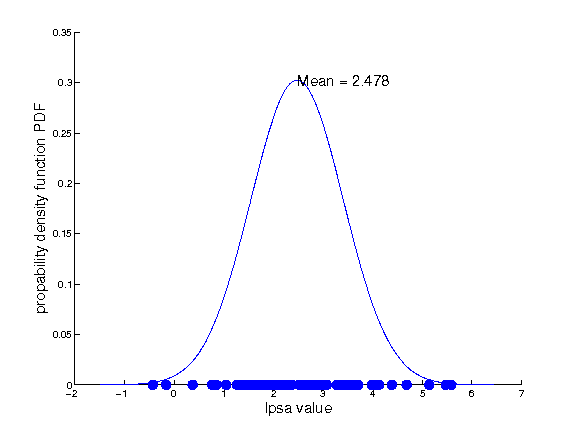
\includegraphics[scale=0.7,bb=0 0 576 432]{output-distribution-tes.png}
		\caption{Verteilung des Outputs (Gauß-modeliert)}
	  \end{subfigure}
	\end{figure}

	\subsubsection*{Source Code}
	
	\verbatiminput{linreg.m} %a


\subsection*{2. Subset Selection}

	Im folgenden die Summe der quadratischen Abweichungen für alle Kombinationen. Gefittet wurde mit den Trainingsdaten, den Fehler haben wir mit Trainings und Testdaten ermittelt:
	\begin{figure}[H]
	  \begin{subfigure}
	    \centering
	    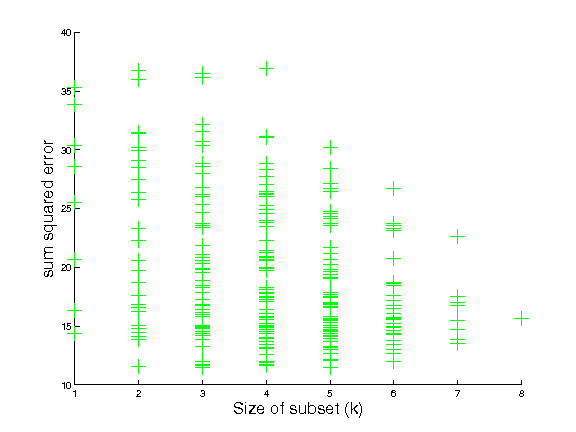
\includegraphics[scale=0.7,bb=0 0 576 432]{task2-sum-sq-errors-tes.png}
		\caption{Summe der quadratischen Abweichungen auf Basis Testdaten}
	  \end{subfigure}
	\end{figure}
	\begin{figure}[H]
	  \begin{subfigure}
	    \centering
	    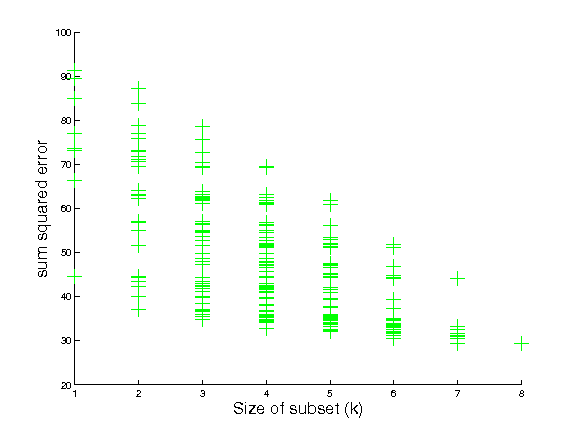
\includegraphics[scale=0.7,bb=0 0 576 432]{task2-sum-sq-errors.png}
		\caption{Summe der quadratischen Abweichungen auf Basis Trainingsdaten}
	  \end{subfigure}
	\end{figure}
	
	Wir haben die Resultate für jedes Größe k des Subsets nach Fehlerrate sortiert (siehe Logfile unten)\\
	Die geringste Fehlerrate hinsichtlich der Testdaten wird mit den drei Features $ \{1, 5, 7\} $ erzielt. Für die Fehlerrate auf den Trainingsdaten ist es optimal alle Parameter zu berücksichtigen. Es wird deutlich was mit dem Overfittings-Problem gemeint ist: Die Hyperebene die mit allen 8 Parametern für die Traningsdaten optimiert wurde hat zwar eine optimale Fehlerrate auf den Trainingsdaten, ist aber schlecht generalisierbar (für Testdaten).\\
	Man sieht außerdem, dass z. B. das Feature 1 für alle k immer in den besten Subsets enthalten ist. Das deckt sich damit, dass Feature 1 scheinbar generell gut mit dem lpsa korreliert (siehe Feature-Plot für 1 ganz am Ende).\\
	Die Reduktion der Merkmale sollte man aber wohl besser mit den in der Vorlesung vorgestellten Algorithmen (z. B. coefficient selection) durchführen.\\
	
	Im Folgenden ein Auszug aus dem Logfile, aus dem die besten Subsets abgelesen werden können:
	\begin{verbatim}
Features		squared-error	Weights
k=1
1	14.392	[1.52 0.713]
6	16.346	[2.54 0.422]
5	20.632	[2.09 1.6]
7	25.530	[-1.48 0.583]
8	28.617	[1.97 0.0185]
2	30.403	[-2.01 1.23]
3	33.847	[0.0795 0.0366]
4	35.299	[2.44 0.217]

k=2
[1 5]	11.584	[1.54 0.604 0.542]
[1 8]	13.828	[1.46 0.655 0.00504]
...

k=3
[1 5 7]	11.484	[1.27 0.595 0.536 0.0411]
[1 5 8]	11.632	[1.5 0.58 0.472 0.00332]
...

k=4
[1 3 5 7]	11.613	[1.12 0.591 0.00373 0.542 0.0291]
[1 2 3 5]	11.636	[-0.642 0.532 0.768 -0.00784 0.529]
...

k=5
[1 2 3 5 7]	11.498	[-1.48 0.503 0.812 -0.0124 0.502 0.151]
...

k=6
[1 2 3 5 7 8]	12.009	[-0.663 0.496 0.812 -0.0121 0.415 0.0114 0.00511]
...

k=7
[1 2 3 4 5 6 7]	13.493	[-0.866 0.556 0.619 -0.0187 0.144 0.803 -0.131 0.198]
...

k=8
[1 2 3 4 5 6 7 8]	15.638	[0.429 0.577 0.614 -0.019 0.145 0.737 -0.206 -0.0295 0.00947]
	\end{verbatim}


	
	
\subsection*{2. Anhang}
	Noch ein paar Ergänzungen (nicht Teil der Aufgabenstellung 2)
	Um ein Gefühl für die tatsächliche Abweichung zu bekommen haben wir die mittlere quadratische und absolute Abweichung berechnet:
	\begin{figure}[H]
	  \begin{subfigure}
	    \centering
	    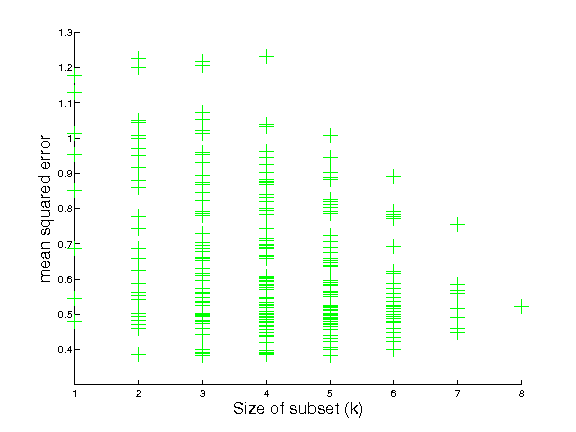
\includegraphics[scale=0.7,bb=0 0 576 432]{task2-mean-sq-errors.png}
		\caption{Mittelwert der quadratischen Abweichungen (Testdaten)}
	  \end{subfigure}
	\end{figure}
	\begin{figure}[H]
	  \begin{subfigure}
	    \centering
	    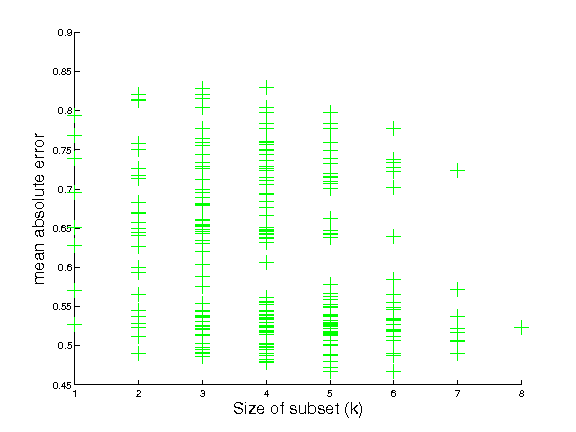
\includegraphics[scale=0.7,bb=0 0 576 432]{task2-mean-abs-errors.png}
		\caption{Mittelwert der absoluten Abweichungen (Testdaten)}
	  \end{subfigure}
	\end{figure}
	Erstaunlicherweise ist dass die absoluten Abweichungen den quadratische Abweichung beinahe vollständig entsprechen. Das liegt wohl daran, dass die Abweichungen mal kleiner, mal größer 0 sind und somit das quadrieren nicht zwangsweise in größeren Zahlen resultiert. Das es fast identisch ist, können wir uns aber nicht wirklich erklären.\\
	
	Außerdem haben wir die lineare Regression für jedes Feature einzeln geplottet:
	\begin{figure}[H]
	  \begin{subfigure}
	    \centering
	    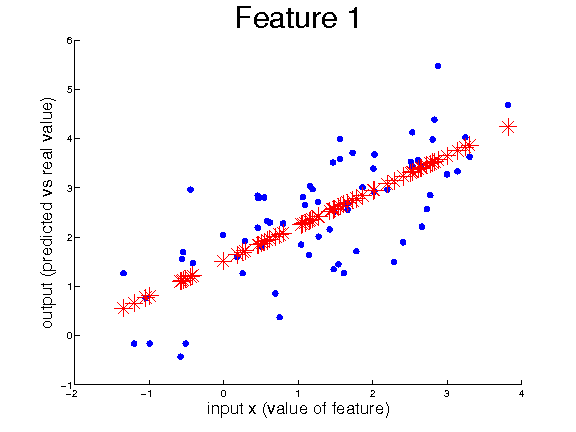
\includegraphics[scale=0.4,bb=0 0 576 432]{task2-feature1.png}
	  \end{subfigure}
	  \begin{subfigure}
	    \centering
	    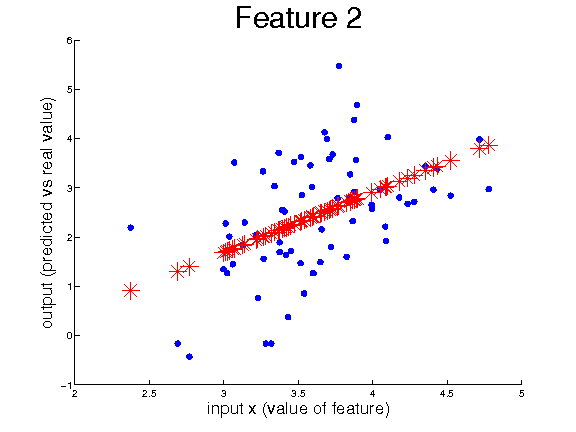
\includegraphics[scale=0.4,bb=0 0 576 432]{task2-feature2.png}
	  \end{subfigure}
	\end{figure}
	\begin{figure}[H]
	  \begin{subfigure}
	    \centering
	    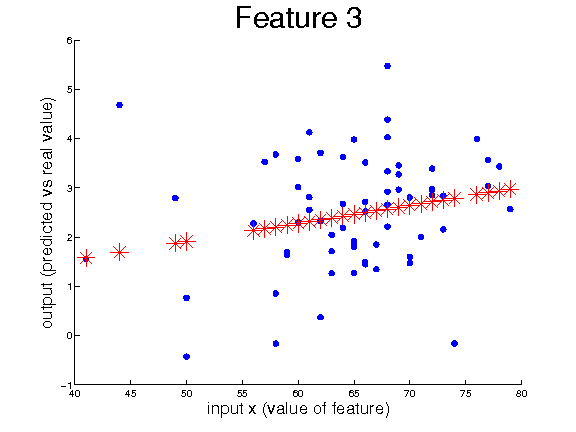
\includegraphics[scale=0.4,bb=0 0 576 432]{task2-feature3.png}
	  \end{subfigure}
	  \begin{subfigure}
	    \centering
	    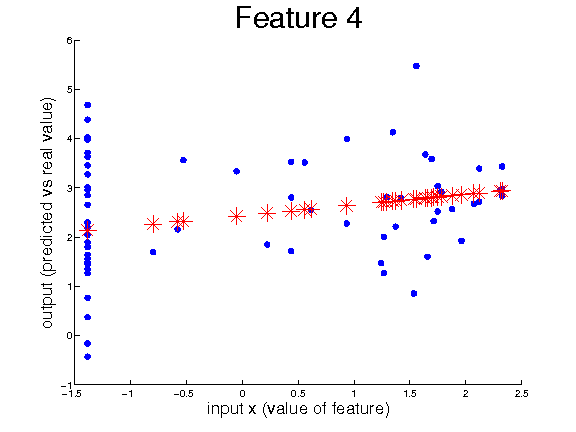
\includegraphics[scale=0.4,bb=0 0 576 432]{task2-feature4.png}
	  \end{subfigure}
	\end{figure}
	\begin{figure}[H]
	  \begin{subfigure}
	    \centering
	    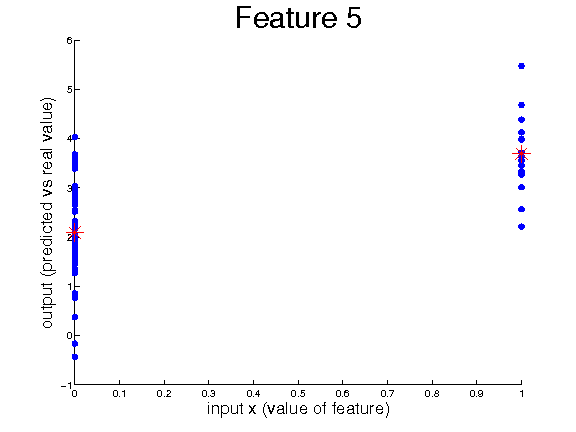
\includegraphics[scale=0.4,bb=0 0 576 432]{task2-feature5.png}
	  \end{subfigure}
	  \begin{subfigure}
	    \centering
	    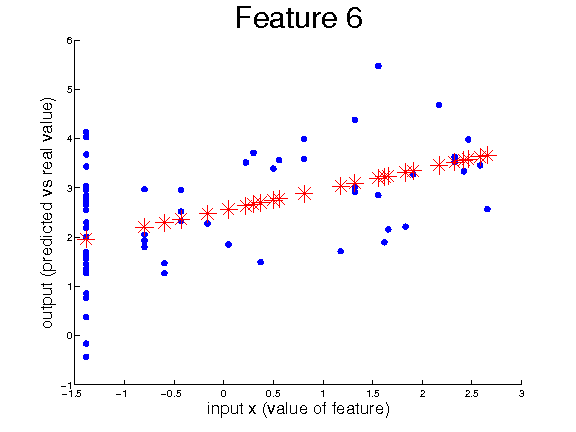
\includegraphics[scale=0.4,bb=0 0 576 432]{task2-feature6.png}
	  \end{subfigure}
	\end{figure}
	\begin{figure}[H]
	  \begin{subfigure}
	    \centering
	    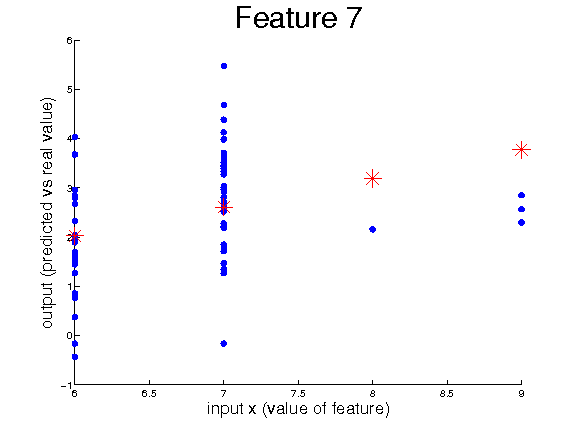
\includegraphics[scale=0.4,bb=0 0 576 432]{task2-feature7.png}
	  \end{subfigure}
	  \begin{subfigure}
	    \centering
	    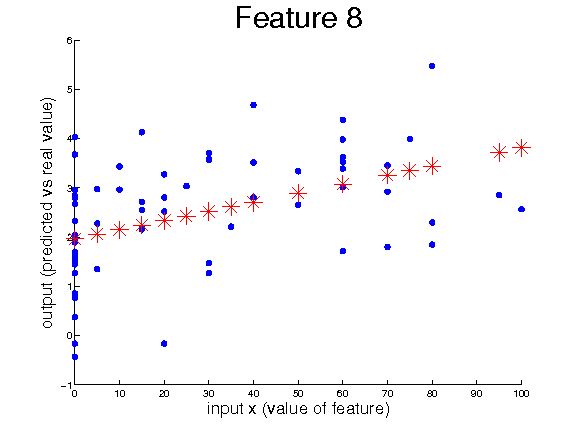
\includegraphics[scale=0.4,bb=0 0 576 432]{task2-feature8.png}
	  \end{subfigure}
	\end{figure}
	
\end{document}
